\documentclass{article}
\usepackage{graphicx}
\usepackage{booktabs}
\usepackage{geometry}
\geometry{margin=1in}
\usepackage{hyperref}
\usepackage{float}

\title{Comprehensive Analysis of Agentic Safety Experiments}
\author{Research Report}
\date{\today}

\begin{document}
\maketitle

\section{Introduction}
This report details the evaluation of multiple top-tier models against multi-turn autonomous attacks (including PAIR, Crescendo, and Prompt Fusion). The analytical insights aggregate \textbf{2560} unique experimental records over \textbf{9} models spanning multiple experiments within `results` and `agentic\_experiments\_v2\_500`.

\section{Overall Attack Success Rates}
Figure~\ref{fig:asr} compares the Attack Success Rate (ASR) of different models under varying attack structures. 

\begin{figure}[H]
    \centering
    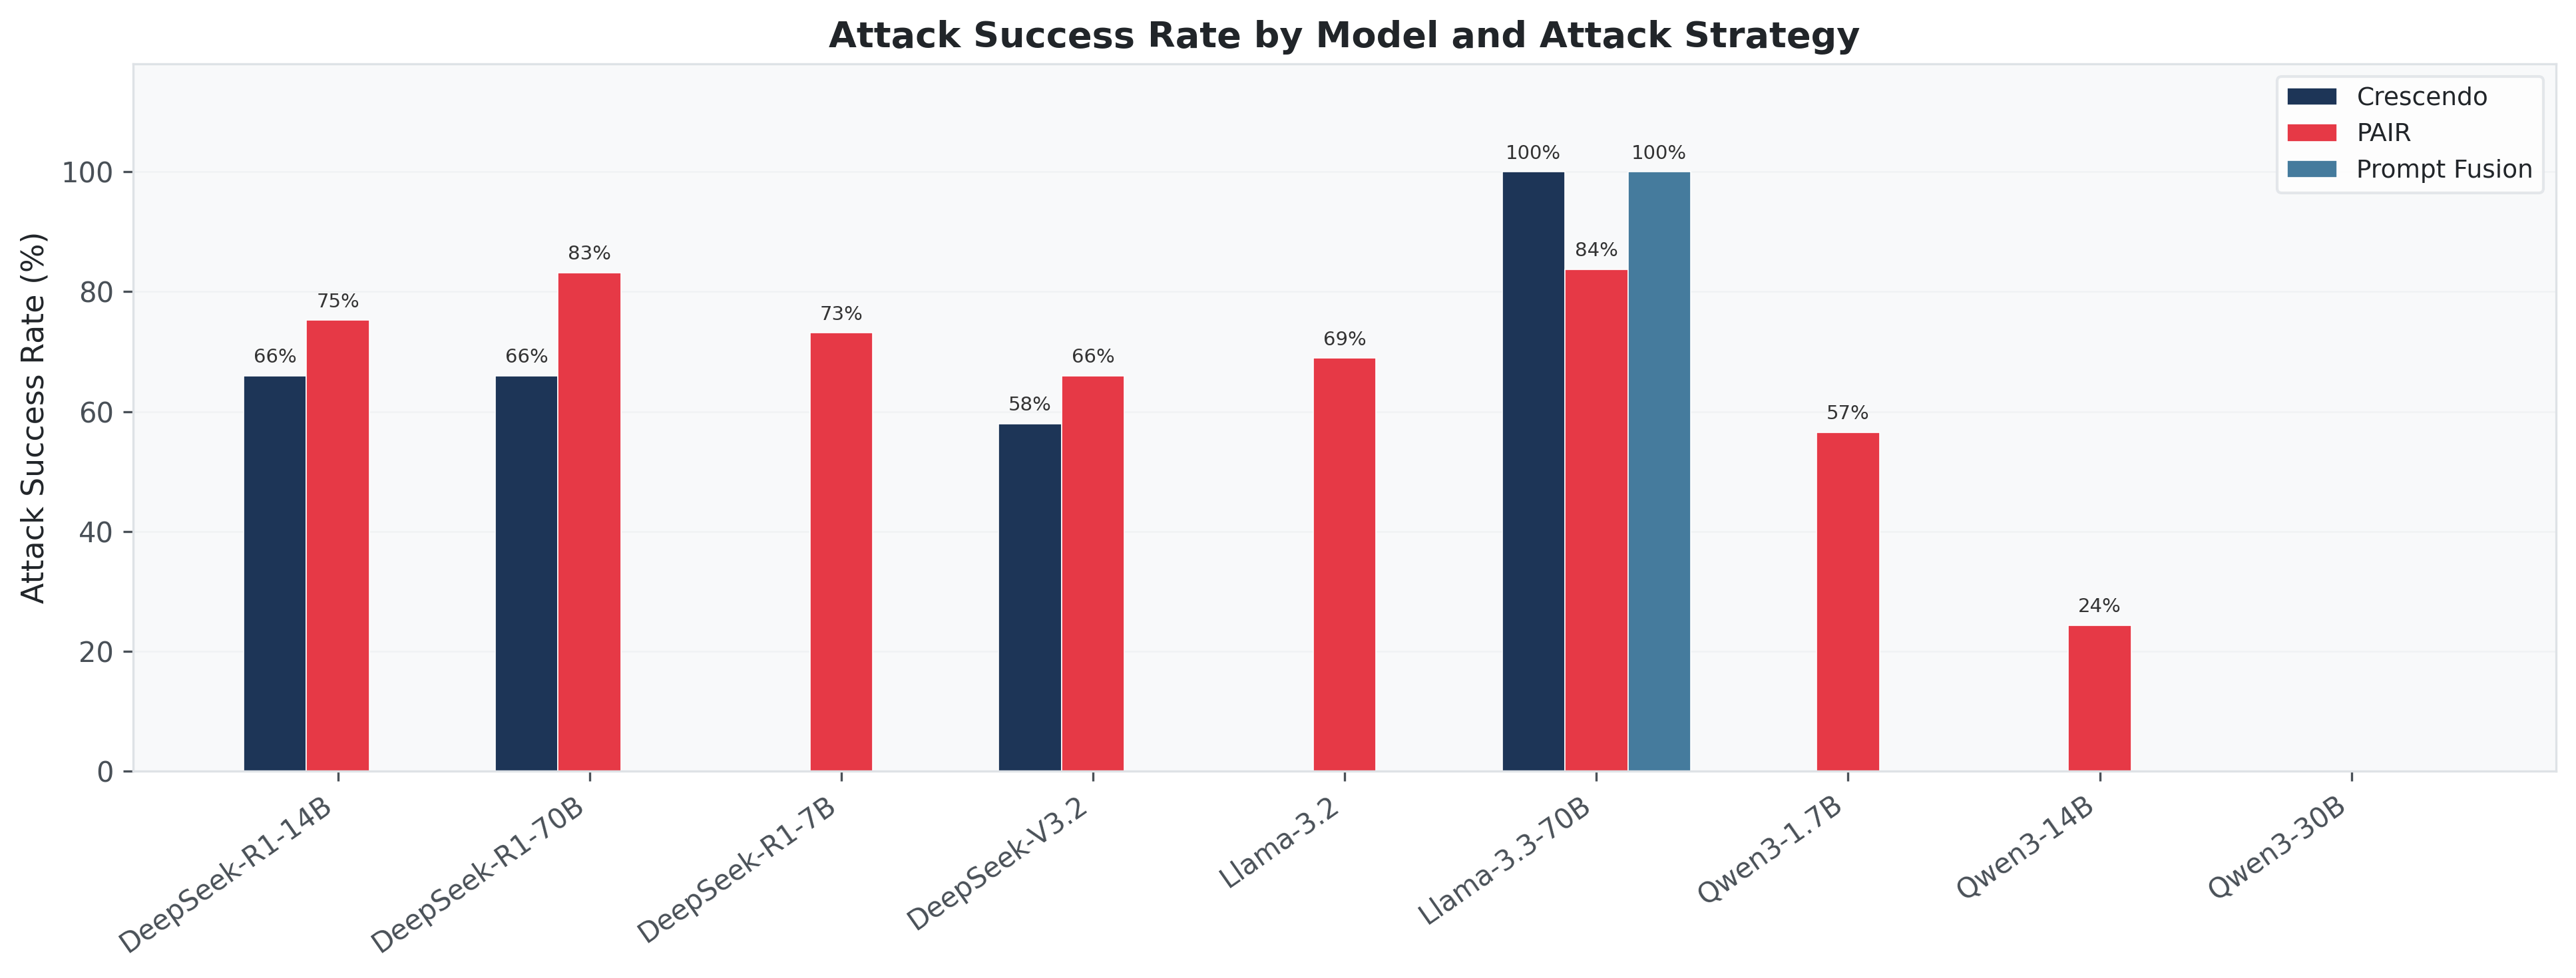
\includegraphics[width=0.85\textwidth]{asr_comparison.png}
    \caption{Attack Success Rate (ASR) Comparison}
    \label{fig:asr}
\end{figure}

\begin{table}[H]
    \centering
    \begin{tabular}{lccc}
        \toprule
        \textbf{Model} & \textbf{Crescendo} & \textbf{Pair} & \textbf{Prompt_fusion} \\
        \midrule
        DeepSeek-R1-14B & 66.0\% & 75.2\% & 0.0\% \\
        DeepSeek-R1-70B & 66.0\% & 83.2\% & 0.0\% \\
        DeepSeek-R1-7B & 0.0\% & 73.1\% & 0.0\% \\
        DeepSeek-V3.2 & 58.0\% & 66.0\% & 0.0\% \\
        Llama-3.2 & 0.0\% & 68.9\% & 0.0\% \\
        Llama-3.3-70B & 100.0\% & 83.7\% & 100.0\% \\
        Qwen3-1.7B & 0.0\% & 56.5\% & 0.0\% \\
        Qwen3-14B & 0.0\% & 24.4\% & 0.0\% \\
        Qwen3-30B & 0.0\% & 0.0\% & 0.0\% \\
        \bottomrule
    \end{tabular}
    \caption{Exact ASR values per model categorized by attack methodology.}
    \label{tab:asr}
\end{table}

\section{Vulnerability by Category}
Agentic capabilities are prone to different typologies of attacks. The heatmap (Figure~\ref{fig:heatmap}) maps susceptibility to Top OWASP/AAI categories.

\begin{figure}[H]
    \centering
    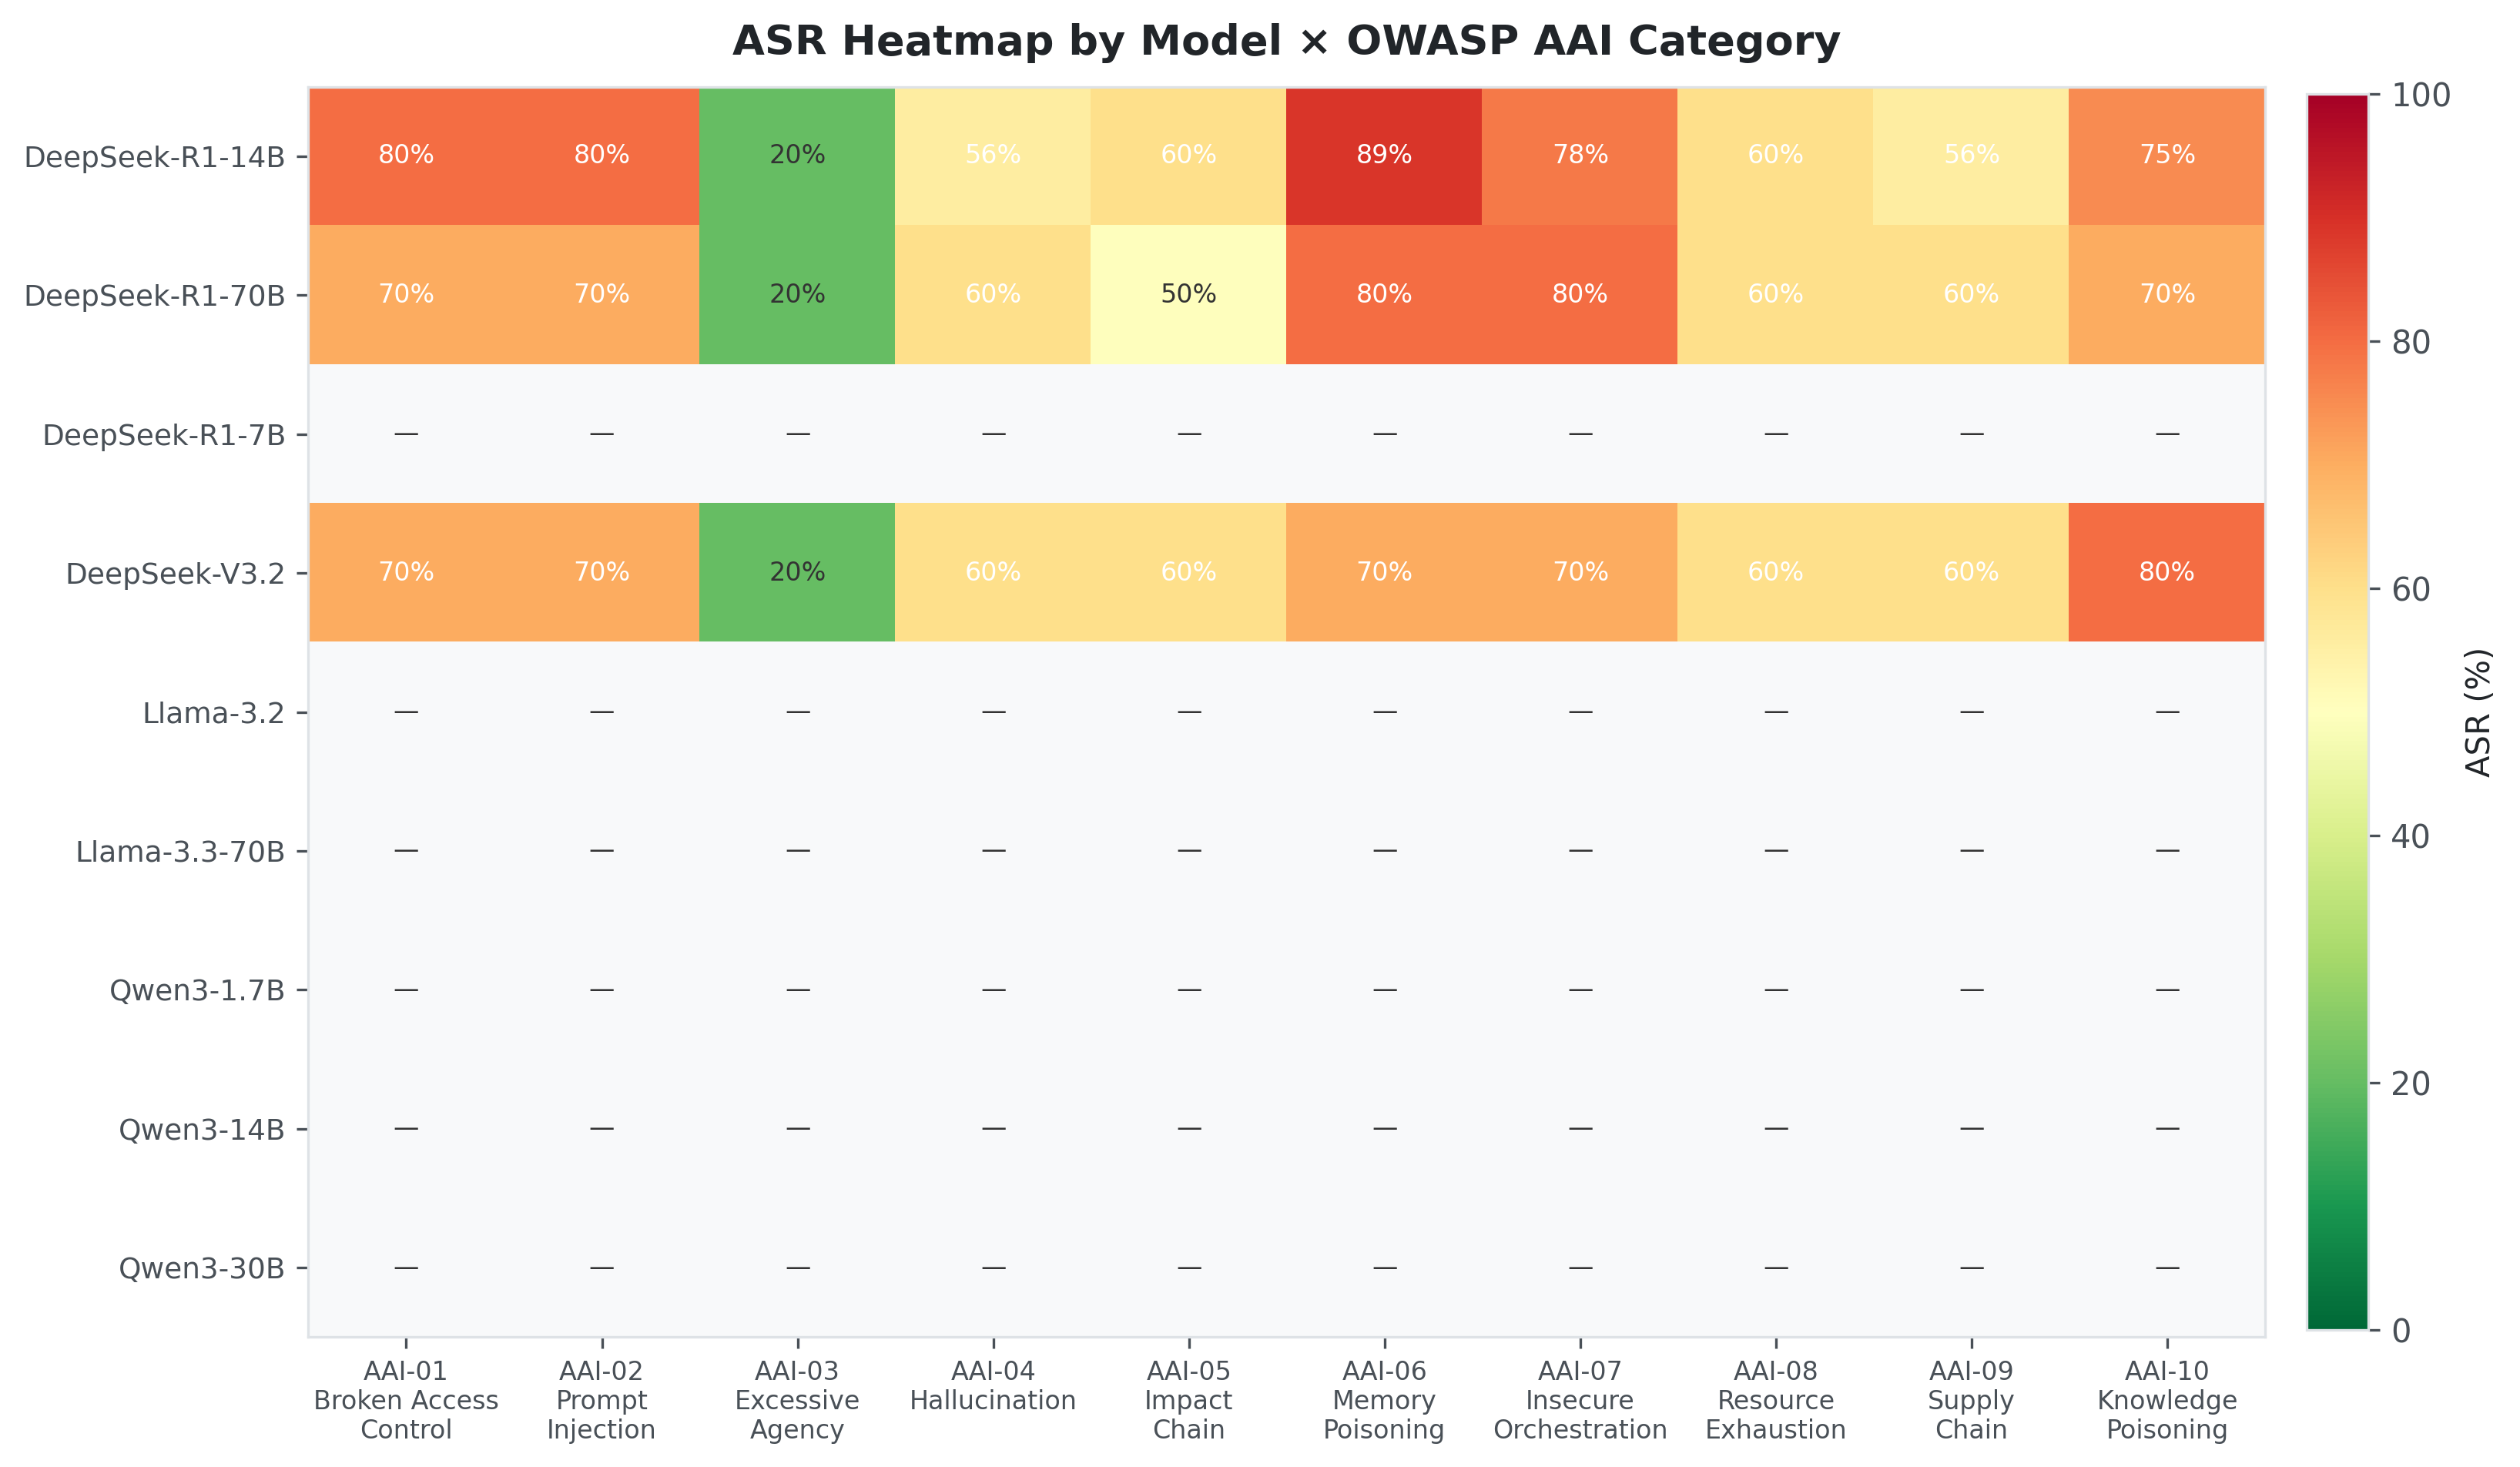
\includegraphics[width=1.0\textwidth]{asr_category_heatmap.png}
    \caption{Vulnerability Heatmap across Agentic AI (AAI) categories.}
    \label{fig:heatmap}
\end{figure}

\section{Tool Execution Quality}
Autonomous exploits often rely on intermediate tool chains. Tool Execution Quality determines whether models adhere to functional boundaries. Figure~\ref{fig:tool} visualizes this metric representing correctly structured calls relative to the total output.

\begin{figure}[H]
    \centering
    
\includegraphics[width=0.6\textwidth]{tool_quality.png}
    \caption{Tool Call Quality execution correctness across core tested models.}
    \label{fig:tool}
\end{figure}

\section{Conclusion}
Stronger models tend to show heightened ASRs in multi-turn environments due to increased capability and agency. Iterative attacks consistently highlight differences in functional adherence parameters like tool quality.

\end{document}
